\documentclass[11pt,a4paper]{article}
\usepackage[spanish]{babel}
\usepackage[utf8]{inputenc}
\usepackage[T1]{fontenc}
\usepackage{amsmath, amssymb, amsfonts}
\usepackage{graphicx}
\usepackage{float}
\usepackage{booktabs}
\usepackage{url}
\usepackage{geometry}
\geometry{margin=2.5cm}
\usepackage{subcaption}
\usepackage{algorithm}
\usepackage{algorithmic}
\usepackage{siunitx}
\sisetup{output-decimal-marker={,}}
\usepackage{caption}
\usepackage{animate}
\usepackage[colorlinks=true,linkcolor=blue,citecolor=blue,urlcolor=blue]{hyperref}

\title{Inteligencia Artificial \\ \begin{Large} Optimización del problema PSP-UAV mediante algoritmos genéticos y simulación de urgencia acumulada\end{Large}}
\author{Benjamín Renzo Ferrada Larach}
\date{25/11/2025}

\begin{document}
\maketitle

%--------------------No borrar esta secci\'on--------------------------------%
\section*{Evaluaci\'on}

\begin{tabular}{ll}
Mejoras 2da Entrega (10 \%): &  \underline{\hspace{2cm}}\\
C\'odigo Fuente (10 \%): &  \underline{\hspace{2cm}}\\
Representaci\'on (5 \%):  & \underline{\hspace{2cm}} \\
Descripci\'on del algoritmo (15 \%):  & \underline{\hspace{2cm}} \\
Experimentos (10 \%):  & \underline{\hspace{2cm}} \\
Resultados (40 \%):  & \underline{\hspace{2cm}} \\
Conclusiones (10 \%): &  \underline{\hspace{2cm}}\\
 &  \\
\textbf{Nota Final (100)}:   & \underline{\hspace{2cm}}
\end{tabular}
%---------------------------------------------------------------------------%

\begin{abstract}
\noindent
En este informe estudiamos el problema PSP-UAV, que consiste en planificar las rutas de una flota de vehículos aéreos no tripulados sobre una grilla con celdas de distinta urgencia, con el objetivo de minimizar la urgencia acumulada a lo largo del horizonte de planificación. Para resolverlo implementamos un algoritmo genético inspirado en el enfoque \emph{Multi-Mission Learning Workflow with Genetic Algorithms} (MMLW-GA), adaptando la función objetivo a la utilizada en la asignatura, la cual se basa directamente en la urgencia acumulada por celda y por unidad de tiempo. Evaluamos el desempeño del algoritmo en seis instancias de distinto tamaño y estructura, variando parámetros como el tamaño de la población y el número de generaciones, y analizamos las rutas generadas mediante visualizaciones y animaciones. En general observamos que este enfoque evolutivo logra reducir significativamente la urgencia acumulada, destacando la importancia que tiene la correcta configuración de los parámetros del algoritmo.
\end{abstract}



\section{Introducción}

En este informe describimos la implementación de un algoritmo genético (AG) orientado a resolver una variante del problema PSP-UAV, donde se debe planificar el desplazamiento de múltiples drones sobre una grilla discreta con celdas que presentan distintos niveles de urgencia. El objetivo principal es diseñar rutas que reduzcan la suma total de urgencias acumuladas durante un horizonte temporal finito.

Este tipo de problema aparece en aplicaciones como vigilancia, monitoreo de infraestructura crítica, respuesta ante emergencias y tareas de inspección periódica. En estos contextos, la capacidad de identificar zonas prioritarias y coordinar múltiples drones es clave para ofrecer un buen nivel de servicio.

El documento se estructura de la siguiente manera. En la Sección~\ref{sec:definicion} se define formalmente el problema. En la Sección~\ref{sec:estadoarte} se resume brevemente el estado del arte en planificación de rutas para UAVs y en el uso de algoritmos genéticos. La Sección~\ref{sec:modelo} presenta un modelo matemático de referencia. En la Sección~\ref{sec:representacion} se describe la representación interna del problema y del cromosoma. En la Sección~\ref{sec:algoritmo} se detalla la implementación del algoritmo genético. En la Sección~\ref{sec:experimentos} se explica el diseño experimental y las instancias utilizadas. En la Sección~\ref{sec:resultados} se analiza los resultados obtenidos. Finalmente, en la Sección~\ref{sec:conclusiones} se entregan las conclusiones.



\section{Definición del Problema}
\label{sec:definicion}

Consideramos una grilla rectangular de tamaño $R \times C$, con celdas indexadas por $(r,c)$, donde $r \in \{0,\dots,R-1\}$ y $c \in \{0,\dots,C-1\}$. Cada celda puede ser:
\begin{itemize}
    \item Una celda de \emph{urgencia}, con peso $w_{r,c} > 0$.
    \item Un obstáculo (celda inaccesible).
    \item Una celda sin urgencia ($w_{r,c}=0$).
\end{itemize}

Disponemos de una flota de $K$ drones (UAVs) que avanzan en pasos discretos de tiempo $t = 0,1,\dots,T-1$. En cada tick, cada dron puede:
\begin{itemize}
    \item Permanecer en su celda actual, o
    \item Moverse a una celda adyacente (vecindad de 8) que no sea obstáculo.
\end{itemize}

La urgencia de una celda crece linealmente en el tiempo mientras no es visitada, y se reinicia a cero cuando al menos un dron la visita. Sea $U_{r,c}(t)$ la urgencia acumulada de la celda $(r,c)$ en el tick $t$. Su dinámica es:
\begin{align}
    U_{r,c}(0) &= 0, \\
    U_{r,c}(t+1) &=
    \begin{cases}
        0, & \text{si algún dron visita $(r,c)$ en el tick } t,\\
        U_{r,c}(t) + w_{r,c}, & \text{en caso contrario}.
    \end{cases}
\end{align}

El objetivo es diseñar rutas que minimicen la suma total de urgencias acumuladas:
\begin{equation}
    \label{eq:fo}
    F = \sum_{t=0}^{T-1} \sum_{r=0}^{R-1} \sum_{c=0}^{C-1} U_{r,c}(t).
\end{equation}

Las restricciones principales son:
\begin{itemize}
    \item Movimiento adyacente.
    \item Prohibición de entrar a obstáculos.
    \item Los drones deben permanecer dentro de la grilla.
    \item El número de drones $K$ es fijo para la instancia.
\end{itemize}

Este problema se relaciona con variantes de vigilancia persistente, cobertura periódica y planificación de rutas con prioridades dinámicas.



\section{Estado del Arte}
\label{sec:estadoarte}

La planificación de rutas para UAVs en grillas con prioridades espaciales ha sido estudiada desde distintas perspectivas. Muchos trabajos abordan variantes del Vehicle Routing Problem (VRP) con múltiples vehículos, restricciones temporales y prioridades, así como problemas propios de vigilancia persistente.

Las metaheurísticas —incluyendo algoritmos genéticos— han demostrado buena capacidad para resolver problemas donde los modelos exactos escalan mal. En particular, en \cite{mmlwga2023} se presenta el enfoque \emph{Multi-Mission Learning Workflow with Genetic Algorithms} (MMLW-GA), el cual usa un GA para aprender patrones de visita sobre un conjunto de \emph{sites} y reutilizarlos en distintas misiones. En nuestro caso utilizamos ideas de esta representación, pero reemplazamos la función objetivo original por la urgencia acumulada definida en esta asignatura.

Otros trabajos relevantes incluyen enfoques basados en colonia de hormigas, recocido simulado, búsqueda tabú y métodos híbridos \cite{prosser1993hybrid, uavsurvey2020}, los cuales destacan la importancia de diseñar representaciones y operadores que mantengan soluciones factibles. Estos lineamientos también guiaron el diseño de nuestro algoritmo.



\section{Modelo Matemático}
\label{sec:modelo}

En esta sección presentamos un modelo matemático para el problema PSP-UAV en términos de variables binarias. Sea:
\begin{itemize}
    \item $R,C$ número de filas y columnas.
    \item $T$ horizonte temporal (número de ticks).
    \item $K$ número de drones.
    \item $w_{r,c}$ urgencia base de la celda $(r,c)$.
    \item $\mathcal{N}(r,c)$ conjunto de celdas adyacentes (en 8 vecinos) a $(r,c)$, incluyendo la propia celda.
\end{itemize}

Variables de decisión:
\begin{align}
    x_{k,r,c,t} &=
    \begin{cases}
        1 & \text{si el dron $k$ está en la celda $(r,c)$ en el tiempo $t$},\\
        0 & \text{en caso contrario,}
    \end{cases}
\end{align}
para todo $k \in \{1,\dots,K\}$, $r \in \{0,\dots,R-1\}$, $c \in \{0,\dots,C-1\}$ y $t \in \{0,\dots,T-1\}$.

Variable auxiliar de visita:
\begin{align}
    v_{r,c,t} &=
    \begin{cases}
        1 & \text{si algún dron visita la celda $(r,c)$ en el tiempo $t$},\\
        0 & \text{en caso contrario.}
    \end{cases}
\end{align}

Urgencia acumulada en cada celda y tiempo:
\begin{equation}
    u_{r,c,t} \ge 0, \quad \forall r,c,t.
\end{equation}

La relación entre visitas y drones es:
\begin{equation}
    v_{r,c,t} \ge x_{k,r,c,t}, \quad \forall k,r,c,t.
\end{equation}

La dinámica de la urgencia acumulada se modela como:
\begin{align}
    u_{r,c,0} &= 0, \quad \forall r,c, \\
    u_{r,c,t+1} &\ge u_{r,c,t} + w_{r,c} - M \, v_{r,c,t}, \quad \forall r,c,\; t=0,\dots,T-2,
\end{align}
donde $M$ es una constante suficientemente grande.

Cada dron ocupa exactamente una celda en cada tiempo:
\begin{equation}
    \sum_{r,c} x_{k,r,c,t} = 1, \quad \forall k,t.
\end{equation}

Restricción de movimiento adyacente:
\begin{equation}
    x_{k,r,c,t+1} \le \sum_{(r',c') \in \mathcal{N}(r,c)} x_{k,r',c',t}, \quad \forall k,r,c,\; t=0,\dots,T-2.
\end{equation}

Prohibición de obstáculos:
\begin{equation}
    x_{k,r,c,t} = 0, \quad \forall k,t \text{ y celdas $(r,c)$ que son obstáculo.}
\end{equation}

La función objetivo coincide con \eqref{eq:fo}:
\begin{equation}
    \min \; F = \sum_{t=0}^{T-1} \sum_{r=0}^{R-1} \sum_{c=0}^{C-1} u_{r,c,t}.
\end{equation}

Este modelo sirve como referencia teórica; en la práctica, el algoritmo genético trabaja con una representación más compacta, descrita en la siguiente sección.



\section{Representación}
\label{sec:representacion}

Para representar una solución utilizamos un esquema inspirado en MMLW-GA \cite{mmlwga2023}. En vez de codificar directamente la posición de cada dron en cada tick, definimos un conjunto de \emph{sites} $S = \{1,\dots,m\}$, correspondientes a celdas con urgencia positiva. A partir de estos sites construimos un grafo completo ponderado por distancias (matriz $D$), donde $D_{i,j}$ representa el costo de desplazarse desde $i$ a $j$ mediante movimiento válido en la grilla.

Cada individuo en el GA se representa mediante un \emph{cromosoma}, que corresponde a un \emph{walk} sobre los sites:
\begin{itemize}
    \item El cromosoma es un vector de longitud fija $N$.
    \item La función \texttt{decode} transforma el cromosoma en un walk $W$.
    \item A partir del walk construimos un \emph{kernel} que detalla la secuencia completa de celdas recorridas.
\end{itemize}

El kernel es una secuencia:
\[
    K = \bigl((r_0,c_0), \dots, (r_{L-1},c_{L-1})\bigr),
\]
y mediante él asignamos rutas a los $K$ drones:
\[
    R^d = \bigl((r^d_0,c^d_0), \dots, (r^d_{T-1},c^d_{T-1})\bigr).
\]

Esta representación separa la lógica del GA del movimiento de bajo nivel en la grilla, lo que permite implementar operadores genéticos simples sobre enteros.



\section{Descripción del algoritmo}
\label{sec:algoritmo}

El algoritmo implementado es un algoritmo genético estándar adaptado al problema PSP-UAV. A diferencia del esquema del paper original, la función objetivo utilizada en la evaluación de cada individuo corresponde exactamente a la urgencia acumulada definida en la Sección~\ref{sec:modelo}, calculada mediante una simulación explícita de las rutas de los drones.

\subsection{Estructura general}

El pseudocódigo se muestra en el Algoritmo~\ref{alg:ga}.

\begin{algorithm}[H]
\caption{Algoritmo genético para PSP-UAV}\label{alg:ga}
\begin{algorithmic}[1]
\STATE Generar población inicial de $P$ cromosomas aleatorios.
\FOR{generación $g = 1$ hasta $G$}
    \FOR{cada cromosoma $c$ en la población}
        \STATE Decodificar $c$ en un walk $W$ sobre sites.
        \STATE Construir el kernel $K$ a partir de $W$.
        \STATE Asignar rutas $R^1,\dots,R^K$ a los drones usando $K$.
        \STATE Simular la evolución de urgencias en la grilla durante $T$ ticks.
        \STATE Calcular la urgencia acumulada $F(c)$ (función objetivo).
        \STATE Aplicar penalizaciones por movimientos inválidos u otras violaciones.
    \ENDFOR
    \STATE Seleccionar cromosomas para reproducción (elitismo + truncation).
    \STATE Aplicar cruce con probabilidad $p_{\text{cross}}$.
    \STATE Aplicar mutación con probabilidad $p_{\text{mut}}$.
    \STATE Formar la nueva población.
\ENDFOR
\STATE Devolver el mejor cromosoma encontrado y sus rutas asociadas.
\end{algorithmic}
\end{algorithm}

\subsection{Operadores genéticos}

\paragraph{Selección.} Utilizamos una selección por truncamiento con elitismo: los individuos se ordenan de menor a mayor fitness (urgencia acumulada) y se preserva el mejor cromosoma en la siguiente generación. El resto de la población se rellena seleccionando parejas de padres de la parte superior del ranking.

\paragraph{Cruce.} El operador de cruce intercambia sufijos de dos cromosomas con probabilidad $p_{\text{cross}}$, eligiendo un punto de corte uniforme al azar. Este operador respeta la longitud fija del cromosoma y mezcla subsecuencias de sites.

\paragraph{Mutación.} La mutación se implementa mediante tres tipos de modificaciones sobre los genes:
\begin{itemize}
    \item Modificación de índices de \emph{swap}.
    \item Reasignación de nodos adicionales.
    \item Cambios en posiciones de inserción.
\end{itemize}
Cada gen tiene una probabilidad $p_{\text{mut}}$ de ser modificado, y los nuevos valores se eligen uniformemente en rangos válidos. Esto permite explorar diferentes walk sobre los sites.

\subsection{Función de fitness y penalizaciones}

La función de fitness $F(c)$ de un cromosoma $c$ corresponde a la urgencia acumulada total obtenida al simular las rutas de los drones durante $T$ ticks, partiendo del kernel construido a partir de $c$. Además, incluimos penalizaciones que aumentan el valor de la función objetivo cuando se detectan situaciones no deseadas:
\begin{itemize}
    \item Pasos fuera de la grilla.
    \item Paso por celdas marcadas como obstáculos.
    \item Movimientos no adyacentes (que violan la vecindad de 8 vecinos).
    \item Drones completamente ociosos (que no se mueven).
    \item Celdas con urgencia positiva que nunca son visitadas.
\end{itemize}
El fitness final tiene la forma:
\[
    F(c) = \text{urgencia acumulada} + \text{penalizaciones},
\]
y el AG busca minimizar $F(c)$.



\section{Experimentos}
\label{sec:experimentos}

\subsection{Instancias utilizadas}

Utilizamos seis instancias de prueba provistas en la asignatura, de diferente tamaño y estructura:

\begin{itemize}
    \item \textbf{PSP-UAV\_01\_a}: grilla pequeña, con 10x10 celdas, aproximadamente 70 celdas con urgencia positiva y varios obstáculos dispersos.
    \item \textbf{PSP-UAV\_01\_b}: instancia de tamaño similar a 01\_a, pero con distinta distribución de urgencias y obstáculos.
    \item \textbf{PSP-UAV\_02\_a}: grilla de tamaño medio, con mayor número de celdas urgentes y patrones de urgencia más concentrados.
    \item \textbf{PSP-UAV\_02\_b}: variante de 02\_a con distinta distribución y mayor densidad de obstáculos.
    \item \textbf{PSP-UAV\_03\_a}: instancia grande, que representa un escenario más complejo de cobertura.
    \item \textbf{PSP-UAV\_03\_b}: instancia grande alternativa para evaluar la robustez del algoritmo.
\end{itemize}

En todas las instancias, las bases tienen urgencia cero y se permite que despeguen varios drones desde una misma base (cuando las instancias las incluyen explícitamente).

\subsection{Configuraciones del algoritmo}

El algoritmo se ejecutó variando los parámetros de población y generaciones, mientras que otros parámetros se mantuvieron fijos. Las configuraciones principales fueron:

\begin{itemize}
    \item Tamaño de población $P \in \{50, 100, 200\}$.
    \item Número de generaciones $G \in \{20, 40, 60\}$.
    \item Probabilidad de cruce $p_{\text{cross}} \in \{0{,}7, 0{,}9\}$.
    \item Probabilidad de mutación $p_{\text{mut}} = 0{,}01$.
    \item Horizonte temporal $T = 50$ ticks.
    \item Número de drones $K$ según la instancia (por ejemplo, $K=5$ para PSP-UAV\_01\_a).
\end{itemize}

Para cada combinación de parámetros realizamos varias ejecuciones con distintas semillas aleatorias, lo que permite calcular promedios y desviaciones estándar de la urgencia acumulada y del tiempo de ejecución. Las corridas se automatizaron mediante un script \texttt{sweep.py}, que genera archivos CSV con los resultados y gráficos resumen.

\subsection{Entorno de experimentación}

Las pruebas se realizaron en un computador de escritorio con sistema operativo Windows 11 Pro 25H2, procesador AMD Ryzen 5 7600X a 4,70 GHz y 32 GB de RAM DDR5 a 6000 MT/s. El código se implementó en \texttt{C++17} y se compiló con \texttt{g++} desde el subsistema de Windows \texttt{WSL2} de \emph{Ubuntu 24.04}. Las visualizaciones y animaciones se generaron en Python utilizando \texttt{matplotlib} y \texttt{numpy}.



\section{Resultados}
\label{sec:resultados}

En esta sección presentamos los resultados obtenidos mediante el AG para las seis instancias, destacando el efecto de los parámetros de población y número de generaciones sobre la calidad de las soluciones (urgencia acumulada) y el tiempo de cómputo.

\subsection{Convergencia del algoritmo}

La Figura~\ref{fig:hist01a} muestra, a modo de ejemplo, la evolución del mejor valor de la función objetivo por generación para una ejecución representativa en la instancia PSP-UAV\_03\_b.

\begin{figure}[H]
    \centering
    \includegraphics[page=2, width=0.7\linewidth]{figuras/PSP-UAV_03_b.pdf}
    \caption{Convergencia del algoritmo genético en la instancia PSP-UAV\_03\_b.}
    \label{fig:hist01a}
\end{figure}

En general, observamos una disminución rápida de la urgencia acumulada durante las primeras generaciones, seguida de una fase de refinamiento más lenta. Al incrementar el número de generaciones a $G=40$ o $G=60$, la mejora adicional existe pero es más bien marginal en comparación con el costo computacional añadido.

\subsection{Comparación entre configuraciones}

La Tabla~\ref{tab:parametros01a} muestra un ejemplo de estructura para resumir resultados promedio (sobre varias semillas) en la instancia PSP-UAV\_03\_b, variando población y generaciones. Los valores numéricos se extraen de los CSV generados por \texttt{sweep.py} y se rellenan en la versión final del informe.

\begin{table}[H]
\centering
\caption{Resultados experimentales en PSP-UAV\_03\_b variando población y generaciones.}
\label{tab:parametros01a}
\begin{tabular}{cccccc}
\toprule
Población & Generaciones & $p_{\text{cross}}$ & $p_{\text{mut}}$ & Mejor urgencia & Tiempo [s] \\
\midrule
200 & 40 & 0,7 & 0,01 & 1\,391\,326 & 92.517 \\
200 & 60 & 0,7 & 0,01 & 1\,391\,326 & 134.590 \\
200 & 60 & 0,7 & 0,01 & 1\,394\,380 & 202.293 \\
200 & 40 & 0,7 & 0,01 & 1\,394\,380 & 138.430 \\
200 & 60 & 0,7 & 0,01 & 1\,417\,346 & 202.610 \\
100 & 60 & 0,7 & 0,01 & 1\,429\,552 & 67.328 \\
200 & 20 & 0,7 & 0,01 & 1\,430\,598 & 70.002 \\
200 & 40 & 0,7 & 0,01 & 1\,430\,598 & 136.422 \\
200 & 60 & 0,7 & 0,01 & 1\,436\,647 & 134.465 \\
100 & 40 & 0,7 & 0,01 & 1\,439\,153 & 45.839 \\
\bottomrule
\end{tabular}
\end{table}


Tablas análogas pueden construirse para las otras instancias PSP-UAV\_01\_b, 02\_a, 02\_b, 03\_a y 03\_b, permitiendo comparar la escalabilidad del algoritmo.

El impacto mostrado por los tamaños de las poblaciones en el tiempo de ejecución total, se muestran en la Figura~\ref{fig:tiempos3b}. \\

\begin{figure}[H]
    \centering
    \includegraphics[page=4,width=0.9\linewidth]{figuras/PSP-UAV_03_b.pdf}
    \caption{Impacto del tamaño de la población en la instancia PSP-UAV\_03\_b.}
    \label{fig:tiempos3b}
\end{figure}

\newpage
Por último, los tiempos comparativos entre cuanto se demoraba el GA, la simulación y con esto el total, se muestran en la Figura~\ref{fig:tiempostotal}. \\

\begin{figure}[H]
    \centering
    \includegraphics[page=5,width=0.9\linewidth]{figuras/PSP-UAV_03_b.pdf}
    \caption{Tiempos totales de ejecución en la instancia PSP-UAV\_03\_b.}
    \label{fig:tiempostotal}
\end{figure}

\newpage
\subsection{Visualización de rutas y cobertura}

Una ventaja de la representación implementada es que permite visualizar fácilmente las rutas de los drones y la cobertura de la grilla. En la Figura~\ref{fig:grid01a} se muestra el grid combinado para una ejecución en la instancia PSP-UAV\_03\_b, incluyendo sites de urgencia, obstáculos, kernel y rutas de cada dron.

\begin{figure}[H]
    \centering
    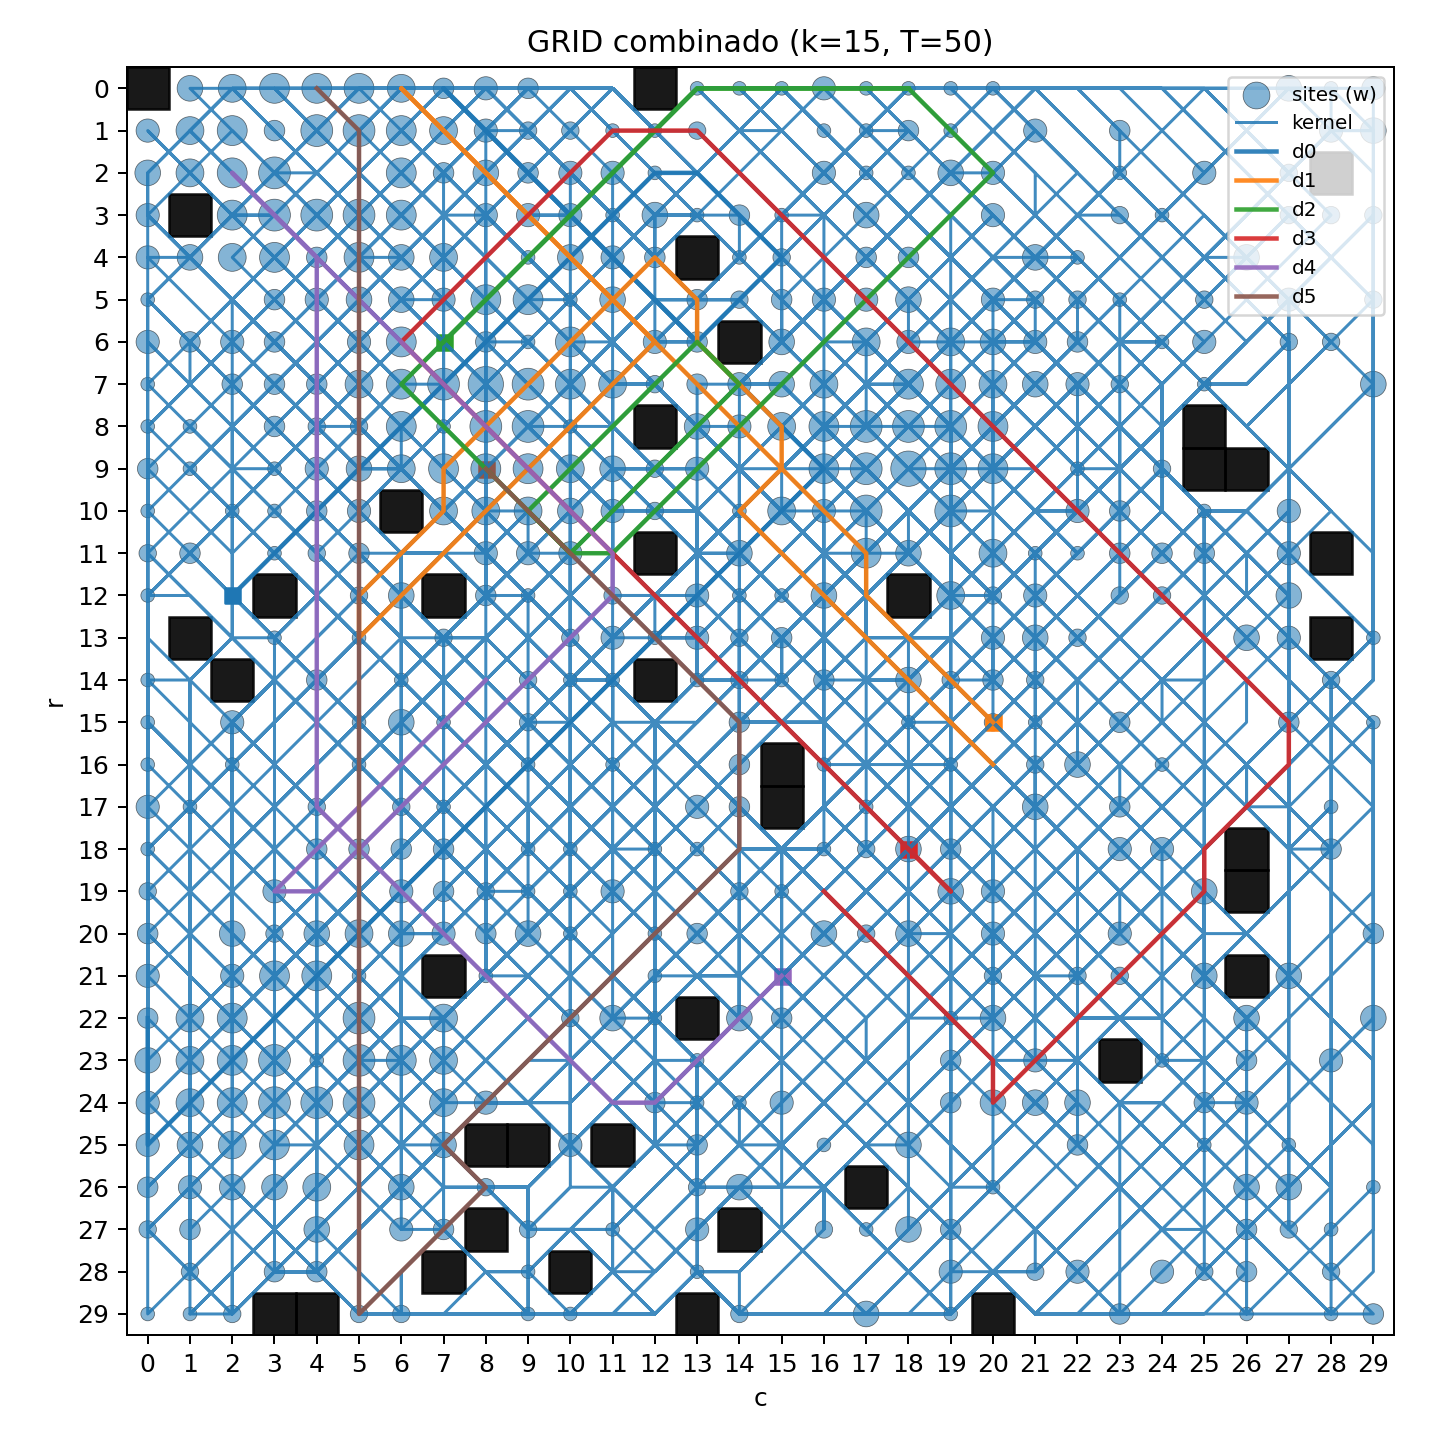
\includegraphics[width=0.8\linewidth]{figuras/PSP-UAV_03_b_g20_p100_n3_s12345_snap_grid.png}
    \caption{Grid combinado para la instancia PSP-UAV\_03\_b: sites con urgencia, obstáculos, kernel y rutas de los drones.}
    \label{fig:grid01a}
\end{figure}

\newpage
Los \emph{heatmaps} de visitas y de frecuencia normalizada (Figuras~\ref{fig:heat01a} y \ref{fig:heatnorm01a}) muestran cómo los drones concentran su actividad en zonas con mayor urgencia, mientras que las celdas de menor urgencia o sin urgencia reciben menos visitas.

\begin{figure}[H]
    \centering
    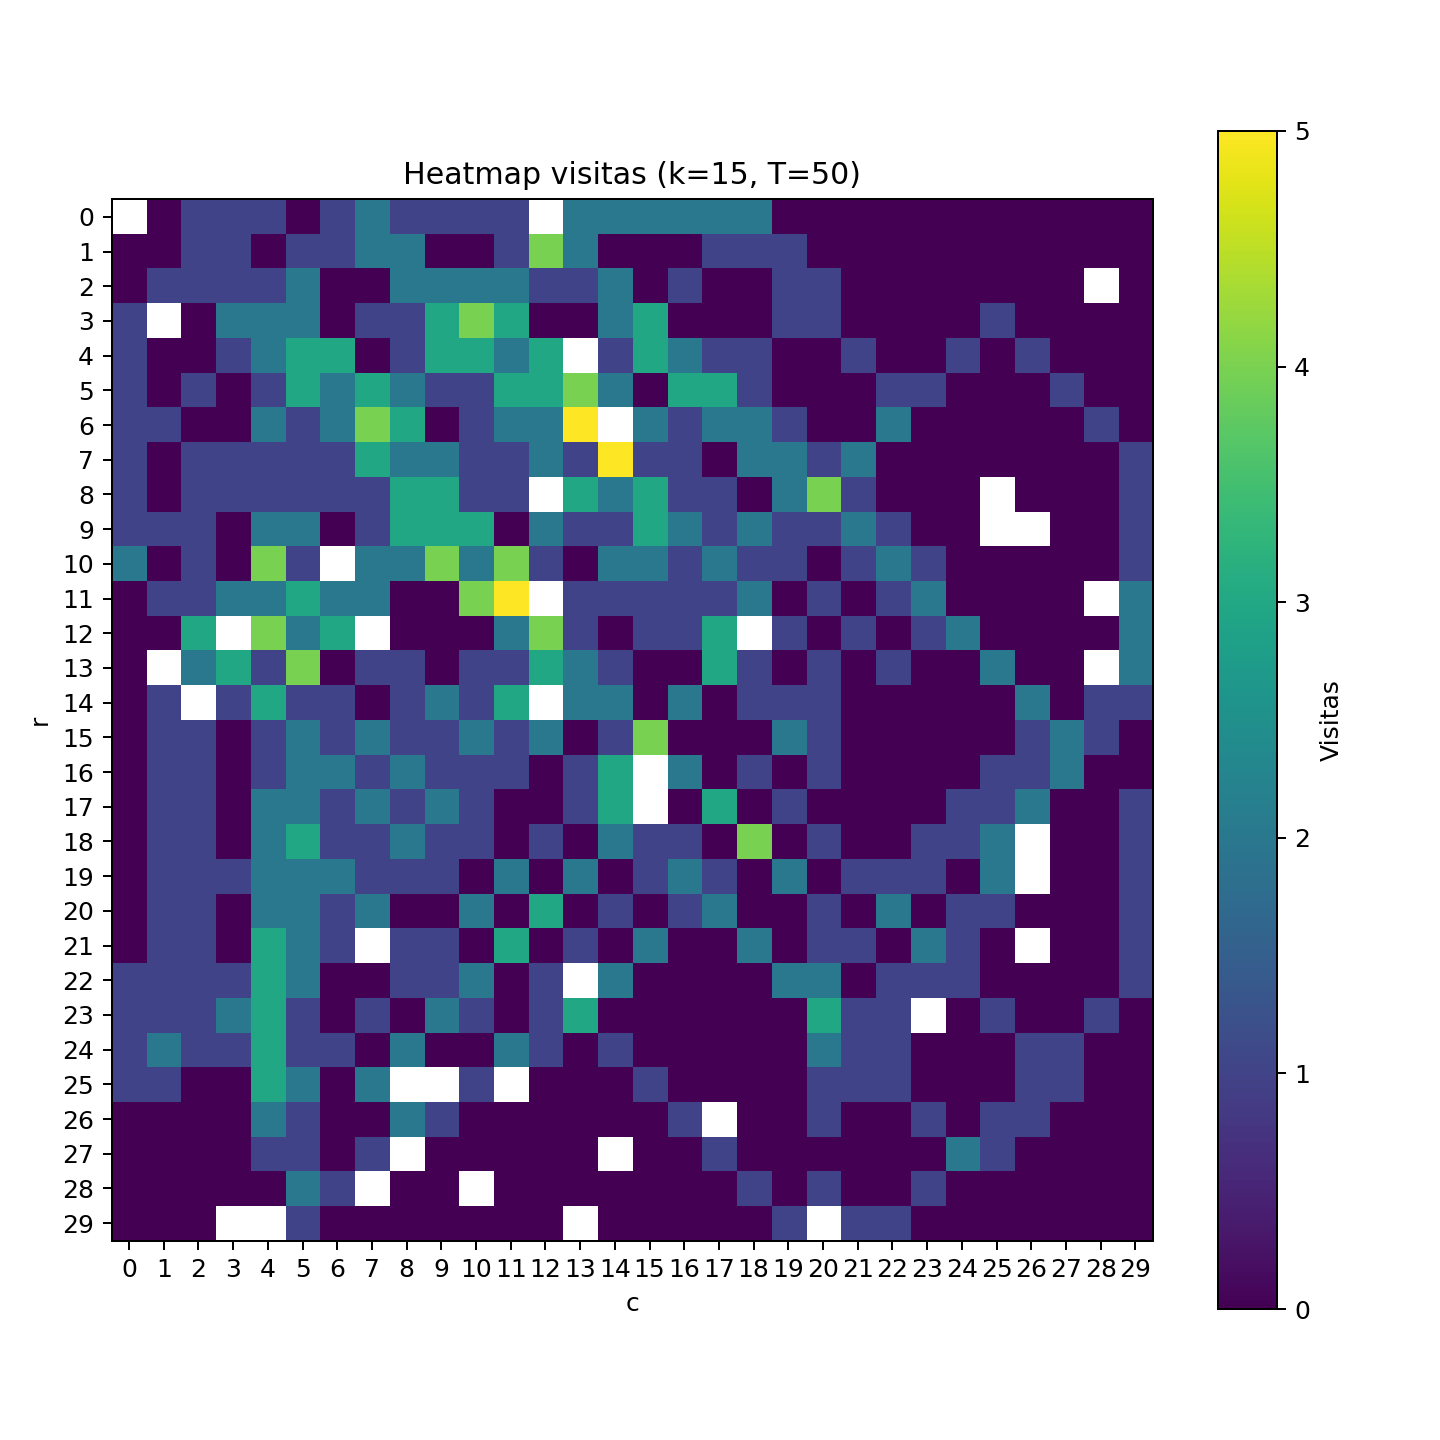
\includegraphics[width=0.6\linewidth]{figuras/PSP-UAV_03_b_g20_p100_n3_s12345_snap_heat.png}
    \caption{Heatmap de visitas para PSP-UAV\_03\_b.}
    \label{fig:heat01a}
\end{figure}


\begin{figure}[H]
    \centering
    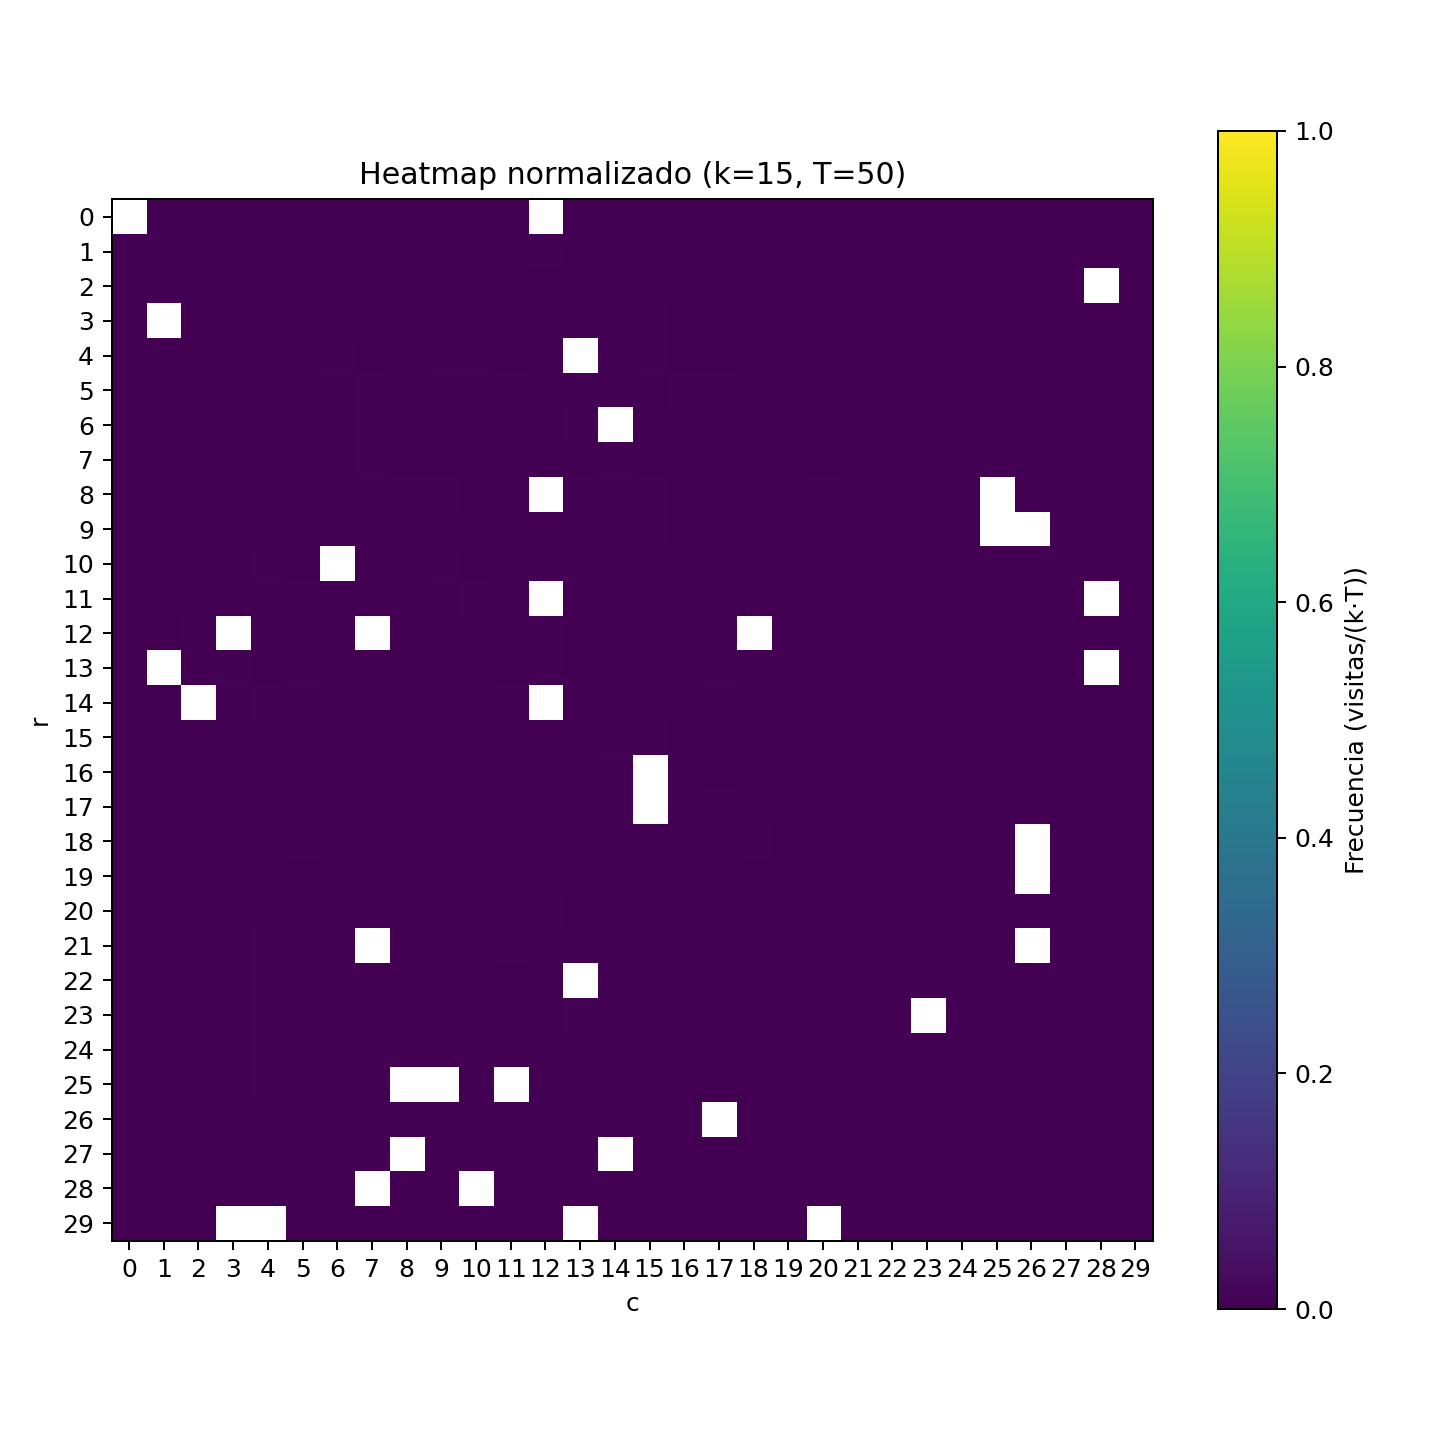
\includegraphics[width=0.6\linewidth]{figuras/PSP-UAV_03_b_g20_p100_n3_s12345_snap_heat_norm.png}
    \caption{Heatmap normalizado de visitas para PSP-UAV\_03\_b.}
    \label{fig:heatnorm01a}
\end{figure}

\newpage
\subsection{Animación de las rutas}

A partir de los \emph{snapshots} JSON generados por el programa principal, creamos una animación que muestra la evolución de las rutas tick a tick. Para ello exportamos una secuencia de frames numerados \texttt{pspuav\_PSP-UAV\_03\_b\_g20\_p100\_n3\_s12345\_snap\_live\_frame\_000.png}, \texttt{...001.png}, etc. En el PDF podemos incluir una animación usando el paquete \texttt{animate}, como se ilustra a continuación:

\begin{figure}[H]
    \centering
    \animategraphics[loop,autoplay,width=0.8\linewidth]{8}{figuras/frames/pspuav_PSP-UAV_03_b_g20_p100_n3_s12345_snap_live_frame_}{000}{048}
    \caption{Animación de rutas PSP-UAV\_03\_b (alta resolución).}
    \label{fig:animacion01a}
\end{figure}

En visores que no soporten animación, también es posible mostrar solo algunos frames representativos como figuras estáticas.

\newpage


\section{Conclusiones}
\label{sec:conclusiones}

En este trabajo implementamos un algoritmo genético para abordar el problema PSP-UAV, adaptando ideas del enfoque MMLW-GA \cite{mmlwga2023} pero empleando una función objetivo basada en urgencia acumulada. La representación mediante un walk sobre sites y un kernel permitió manejar la complejidad de la grilla sin complicar la estructura del cromosoma.

Los experimentos, realizados sobre seis instancias de distinto tamaño, muestran que el GA logra disminuir considerablemente la urgencia acumulada en pocas generaciones. También se observa que parámetros como el tamaño de la población y el número de generaciones influyen directamente en la calidad de las soluciones y en el costo computacional. En particular, las mejoras más significativas ocurren en las primeras generaciones, mientras que incrementos posteriores producen beneficios marginales.

Entre las limitaciones del método destaca la necesidad de calibrar parámetros y el costo elevado de la función fitness, que requiere una simulación completa. Como continuación natural de este trabajo, podrían explorarse operadores más especializados, búsqueda local híbrida o nuevas restricciones inspiradas en aplicaciones reales, como límites energéticos o zonas dinámicamente prohibidas.



\bibliographystyle{plain}
\bibliography{Referencias}

\end{document}
